\newprob{1715607598}
{
    % active phys p107 q2
    一個振動器在一條繩子上產生一個橫向駐波。在 圖示的一刻,所有質點的位移達至其最大值。
    \par{\par\centering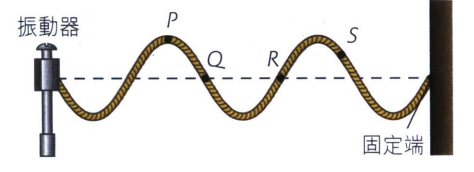
\includegraphics[width=.4\textwidth]{./img/ch3_earlyclass_wave_mc_2024-05-14-10-05-41.png}\par}
    在圖示的一刻,
    \begin{tasks}
        \task 質點$P$正向下移。
        \task 質點 $Q$正向上移。
        \task 質點 $R$正向右移。
        \task 質點$S$ 正在靜止。
    \end{tasks}

}{
    \mckey{D}
    在駐波上,當一顆質點的位移最大,所有質點也是靜止不動的。
}

\newprob{1715652445}
{
    % q3
    把一條繩子拉直,兩端分別固定在相距32 cm 的 $A$、$B$兩點。三枚紙游碼放在繩子上,如圖。
    \par{\par\centering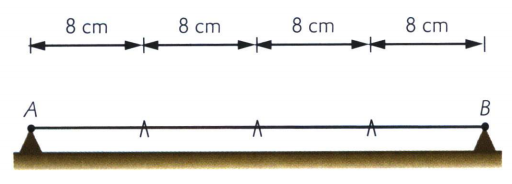
\includegraphics[width=.4\textwidth]{./img/ch3_earlyclass_wave_mc_2024-05-14-10-08-15.png}\par}
    一個駐波在繩子上產生,只有在中間的一枚游碼 沒有掉下來。波的波長可能為多少?
    \begin{tasks}
        \task \qty{8}{cm}
        \task \qty{16}{cm}
        \task \qty{24}{cm}
        \task \qty{32}{cm}
    \end{tasks}

}{\mckey{D}}

\newprob{1715652605}
{
    % q4
    一個橫向駐波在一條兩端固定的繃緊繩子上形 成。以下哪一項敘述必定正確?
    \begin{tasks}
        \task 能量從繩子一端傳遞至另一端。
        \task 繩子上所有的質點不停振動。
        \task 繩子上不同位置的質點有不同的振幅。
        \task 繩子上波腹的位置隨時間改變。
    \end{tasks}

}{
    \mckey{C}
}

\newprob{1715652700}
{
    % active phys p101 q1
    兩個相干的波源$S$,和$S$,產生同相的聲波,波長 為2 cm。
    \par{\par\centering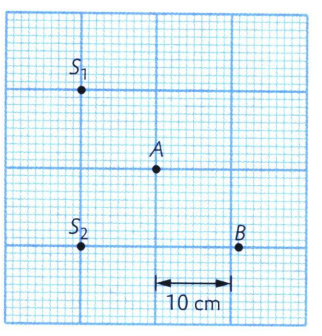
\includegraphics[width=.3\textwidth]{./img/ch3_earlyclass_wave_mc_2024-05-14-10-28-28.png}\par}
    在$A$點和$B$ 點分別發生哪一種干涉現象?
    \begin{tasks}
        \task \textbf{A} \tab\tab \textbf{B}
        \task 相長干涉 \tab\tab 相消干涉
        \task 相消干涉 \tab\tab 相長干涉
        \task 相長干涉 \tab\tab 相長干涉
        \task 相消干涉 \tab\tab 相消干涉
    \end{tasks}


}{\mckey A}

\newprob{1715653932}
{
    兩個相干的點振源在水面上產生水波,形成一個 干涉圖案。改變以下哪一項不會影響相長干涉發 生的位置?
    \begin{tasks}

        \task 水波的振幅
        \task 水波的波長
        \task 點振源間的距離
        \task 點振源的振動頻率
    \end{tasks}
}{\mckey A}

\newprob{1715653938}
{
    一列直線水波向一個直線障礙物傳播,障礙物上 有兩道縫隙,如圖。在$A$ 點正發生相消干涉。
    \par{\par\centering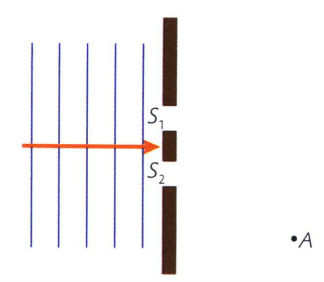
\includegraphics[width=.3\textwidth]{./img/ch3_earlyclass_wave_mc_2024-05-14-11-08-33.png}\par}
    若波長減半,並在$A$ 點發生干涉,以下哪一項 敍述正確?
    \begin{tasks}
        \task 在$A$ 點發生相消干涉。
        \task 在$A$ 點發生相長干涉。
        \task 在$A$ 點總是形成波峯。
        \task 在$A$ 點總是形成波谷。
    \end{tasks}

}{\mckey B}


\newprob{1715659481}
{
    % active p125(109) q2
    以下哪些有關一根繩上的行波和駐波內的質點的 敍述正確?
    \begin{statements}
        \task 所有質點的位移均大於零。
        \task 每一對相隔$\lambda/2$的質點均為反相。(其中$\lambda$為 波長)
        \task 在一個週期內,所有質點均有機會靜止不動。
    \end{statements}
    \begin{tasks}
        \task 只有(1)
        \task 只有(2)
        \task 只有(3)
        \task 以上都不正確
    \end{tasks}
}{\mckey C}

\newprob{1715659634}
{
    % q3
    一個大提琴的弦線長度為$L$,兩端固定。若有駐 波在弦線上形成,下列哪項不可能為波的波長?
    \begin{tasks}
        \task $\dfrac{L}{3}$
        \task $\dfrac{L}{5}$
        \task $\dfrac{2L}{3}$
        \task $\dfrac{3L}{4}$
    \end{tasks}

}{
    \mckey D
}

\newprob{1715659733}
{
    % q4
    銘基藉改變振動器的頻率$f$,在一條一端固定的繩 子上先後產生多個不同的駐波。
    \par{\par\centering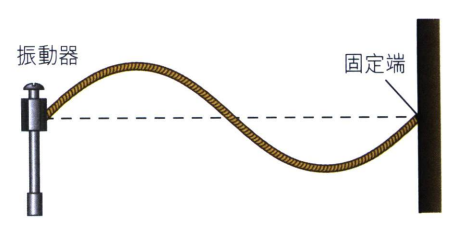
\includegraphics[width=.35\textwidth]{./img/ch3_earlyclass_wave_mc_2024-05-14-12-09-36.png}\par}
    以下哪些敍述是\textbf{不正確}的?
    \begin{tasks}
        \task 當$f$增加,波腹的數目也會增加。
        \task 當$f$減少,繩子上的波速率維持不變。
        \task 繩子在空氣中產生的波,其速率與繩子上的 波速率必定相同。
        \task 除連接至振動器的繩子一端外,波腹與波節 的數目相同。
    \end{tasks}

}{\mckey C}

\newprob{1715660522}
{
    % q5
    一列直線水波從區域 $A$ 傳播至區域 $B$。
    \par{\par\centering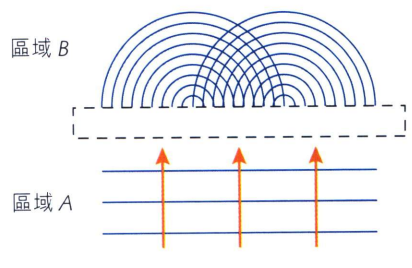
\includegraphics[width=.4\textwidth]{./img/ch3_earlyclass_wave_mc_2024-05-14-12-22-59.png}\par}
    圖中顯示波的哪些特性?(兩個區域間的邊界沒有 顯示出來。)
    \begin{statements}
        \task 折射
        \task 繞射
        \task 干涉
    \end{statements}
    \begin{tasks}
        \task 只有(1)和(2)
        \task 只有(1)和(3)
        \task 只有(2)和(3)
        \task (1), (2) 和 (3)
    \end{tasks}
}{\mckey D}

\newprob{1715660648}
{
    % q6   
    一列直線水波向一個有兩道縫隙的直線障礙物傳 播,在障礙物的另一邊產生兩列圓形波。
    \par{\par\centering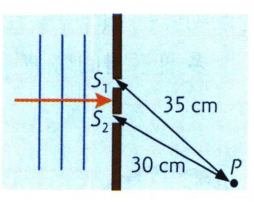
\includegraphics[width=.3\textwidth]{./img/ch3_earlyclass_wave_mc_2024-05-14-12-25-51.png}\par}
    若水面上有一點$P$正發生相長干涉,問下列哪項 不可能為波的波長?
    \begin{tasks}
        \task \qty{0.2}{m}
        \task \qty{2}{m}
        \task \qty{2.5}{m}
        \task \qty{5}{m}
    \end{tasks}

}{\mckey B}
\newprob{1715660647}
{
    % q7
    兩個完全相同的揚聲器$S_1$和$S_2$連接至相同的訊 號。圖中的圓形表示所產生的聲波波陣面。
    \par{\par\centering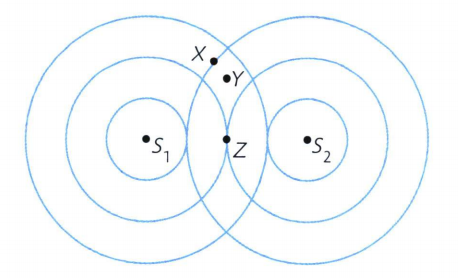
\includegraphics[width=.4\textwidth]{./img/ch3_earlyclass_wave_mc_2024-05-14-12-27-18.png}\par}
    若把$S_2$關掉,在$X$、$Y$和$Z$三點聽到的聲音有甚 麼變化?
    \begin{tasks}
        \task [] \textbf{X} \tab\tab \textbf{Y} \tab\tab \textbf{Z}
        \task 較弱 \tab\tab 較弱 \tab\tab 較響
        \task 較弱 \tab\tab 較響 \tab\tab 較響
        \task 較響 \tab\tab 較響 \tab\tab 較弱
        \task 較響 \tab\tab 較弱 \tab\tab 較弱
    \end{tasks}
}{\mckey{D}}

\newprob{1715660650}
{
    % q8
    德仁站在兩個揚聲器$P$和$Q$前方的$Y$點,並與兩 個揚聲器的距離相等,如圖。
    \par{\par\centering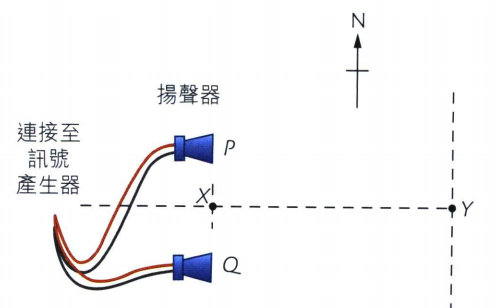
\includegraphics[width=.4\textwidth]{./img/ch3_earlyclass_wave_mc_2024-05-14-12-29-34.png}\par}
    以下各項敍述乃關於德仁聽到的聲音,哪一項是 \textbf{不正確}的?
    \begin{tasks}
        \task 若德仁向南走,則會輪流聽到響亮和微弱的 聲音。
        \task 若德仁向東走,則會一直聽到響亮的聲音。
        \task 若德仁向西北走,則會輪流聽到響亮和微弱 的聲音。
        \task 若其中一個揚聲器斷線,德仁聽到的聲音保 持不變。
    \end{tasks}

}{\mckey D}
\newprob{1715660649}
{
    % q9
    兩個完全相同的揚聲器5,和S,連接至相同的訊 號。曼華手持微音器沿直線PQ移動,發現連續 錄得較響亮聲音的位置為P、O和Q三點。
    \par{\par\centering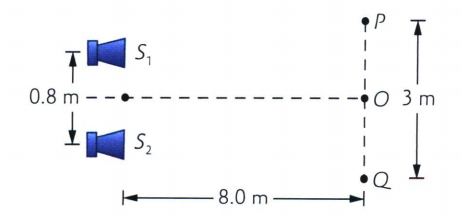
\includegraphics[width=.4\textwidth]{./img/ch3_earlyclass_wave_mc_2024-05-14-13-16-30.png}\par}
    試估計所發出的聲音波長。
    \begin{tasks}
        \task \qty{5}{cm}
        \task \qty{10}{cm}
        \task \qty{15}{cm}
        \task \qty{20}{cm}
    \end{tasks}
}{\mckey C}


\newprob{1715664182}
{
    % active p131(115) *q2
    兩個波源$S_1$和$S_2$相距 1 m,如圖示般在一個平 面上產生波長為0.5 m的 圓形波。
    \par{\par\centering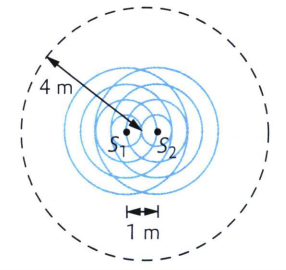
\includegraphics[width=.25\textwidth]{./img/ch3_earlyclass_wave_mc_2024-05-14-13-23-18.png}\par}
    在圖中,有一個半徑為4 m 的圓形,其邊界上可 找到多少個位置發生相長干涉?
    \begin{tasks}
        \task 4
        \task 6
        \task 8
        \task 10
    \end{tasks}

}{\mckey{C}
    \par{\par\centering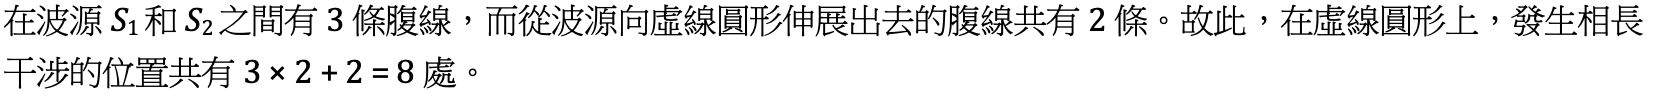
\includegraphics[width=\textwidth]{./img/ch3_earlyclass_wave_mc_2024-05-14-13-24-29.png}\par}
}

\newprob{1715664273}
{
    % q3
    在一個水波槽中,兩個振動的點振源$S_1$和$S_2$產生圓形波,波長分別為$2\lambda$和$\lambda$。下圖顯示$t=0$ 時的波動圖案。實線表示波峯。
    \par{\par\centering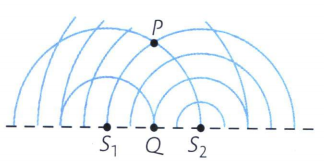
\includegraphics[width=.35\textwidth]{./img/ch3_earlyclass_wave_mc_2024-05-14-13-24-57.png}\par}
    以下哪一項敍述是\textbf{不正確}的?
    \begin{statements}
        \task 由於波長不同,因此波的疊加原理在$P$點並 不適用。
        \task 在$Q$點,波的疊加原理依然適用,但兩個波 不會時時互相抵消。
        \task $P$ 點和$Q$ 點以同相振動。
    \end{statements}
    \begin{tasks}
        \task 只有(1)
        \task 只有(2)
        \task 只有(1)和(3)
        \task 只有(2)和(3)
    \end{tasks}
}{
    \mckey{A}
    \par{\par\centering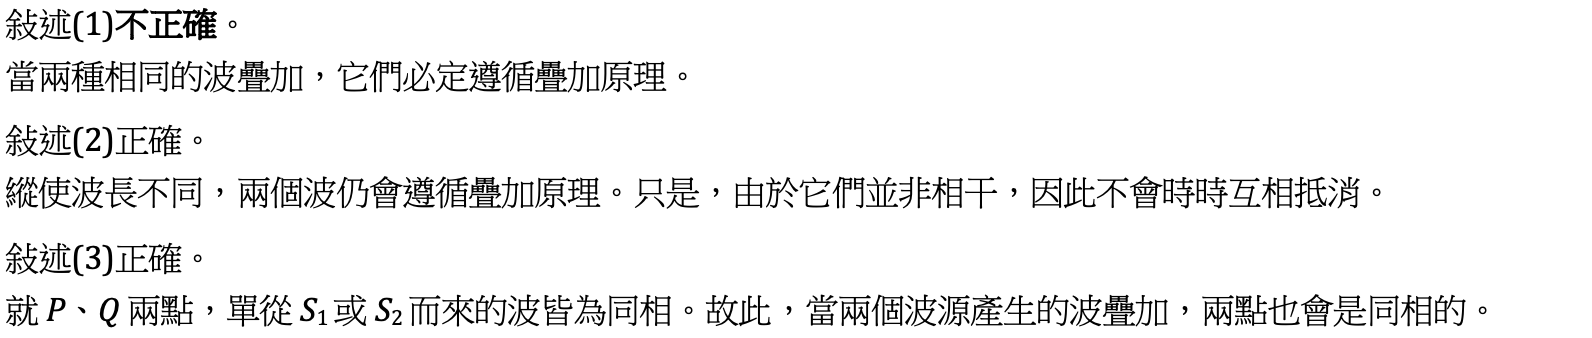
\includegraphics[width=\textwidth]{./img/ch3_earlyclass_wave_mc_2024-05-14-13-31-18.png}\par}
}

\newprob{1715664872}
{
    % *q4
    兩個點振源$S_1$和$S_2$在水面上以同相振動,頻率 為$f$。圖$a$ 表示所形成的腹線與節線位置(分別以 實線和虛線表示)。水面上有一個位置$Q$。圖$b$顯 示由$S$,所造成$Q$點位置的水位的$s$-$t$線圖。
    \par{\par\centering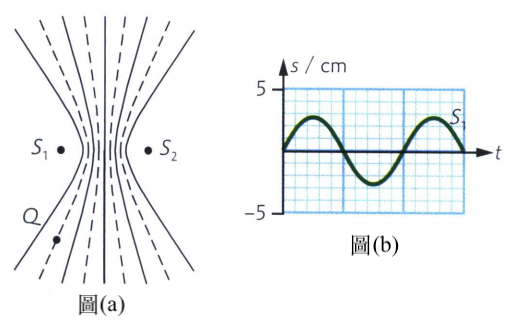
\includegraphics[width=.5\textwidth]{./img/ch3_earlyclass_wave_mc_2024-05-14-13-36-06.png}\par}
    若頻率減少至$f/2$,在Q點的振幅會怎樣改變?
    \begin{tasks}
        \task 變為零
        \task 變得大於 2.5 cm
        \task 變得小於2.5 cm
        \task 不能判斷
    \end{tasks}

}{
    \mckey{B}
    \par{\par\centering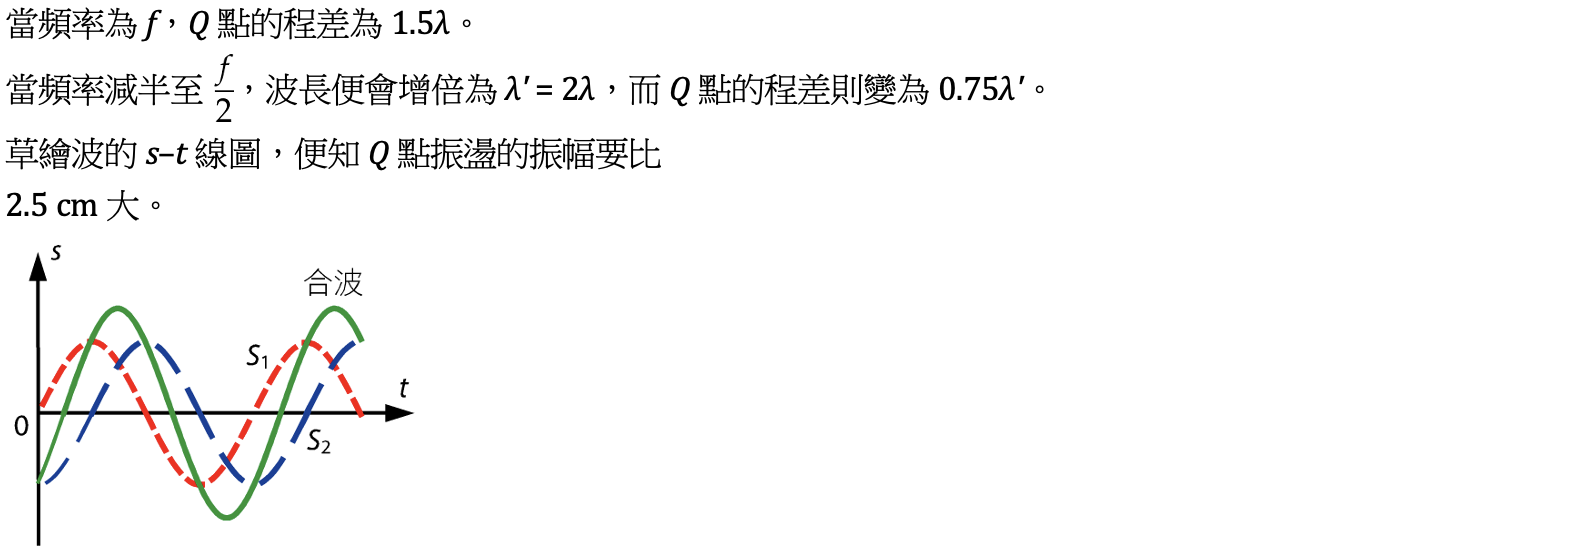
\includegraphics[width=\textwidth]{./img/ch3_earlyclass_wave_mc_2024-05-14-13-37-37.png}\par}
}
